\section{Experiments}
\label{sec:experiments}

This section presents a series of experiments designed to investigate the relationship between learned 3D representations and topology. Our goal is to understand whether and how transformer models capture topological features of shapes, when trained on standard 3D data. We progressively move from a direct evaluation of encoded topology to more indirect analyses. Throughout these experiments, we use DONUT as the main benchmark.

We first conduct a probing analysis to estimate how much topological information can be linearly decoded from the representations of different layers (Section~\ref{ssec:model_probing}). This experiment provides an initial view of the presence and organization of topological cues inside the network. We then study the alignment between the learned embedding space and topological structures derived from persistent homology (Section~\ref{ssec:ph}). This second analysis gives a more geometric perspective on how representations relate to the shape topology. Finally (Section~\ref{ssec:changing_pretraining_data_distribution}), we investigate how changing the pretraining data distribution affects these findings, showing that current pretraining corpora do not explicitly encourage the capture of topological structures.

\subsection{Model Probing}
\label{ssec:model_probing}

\begin{figure}[h]
  \centering
  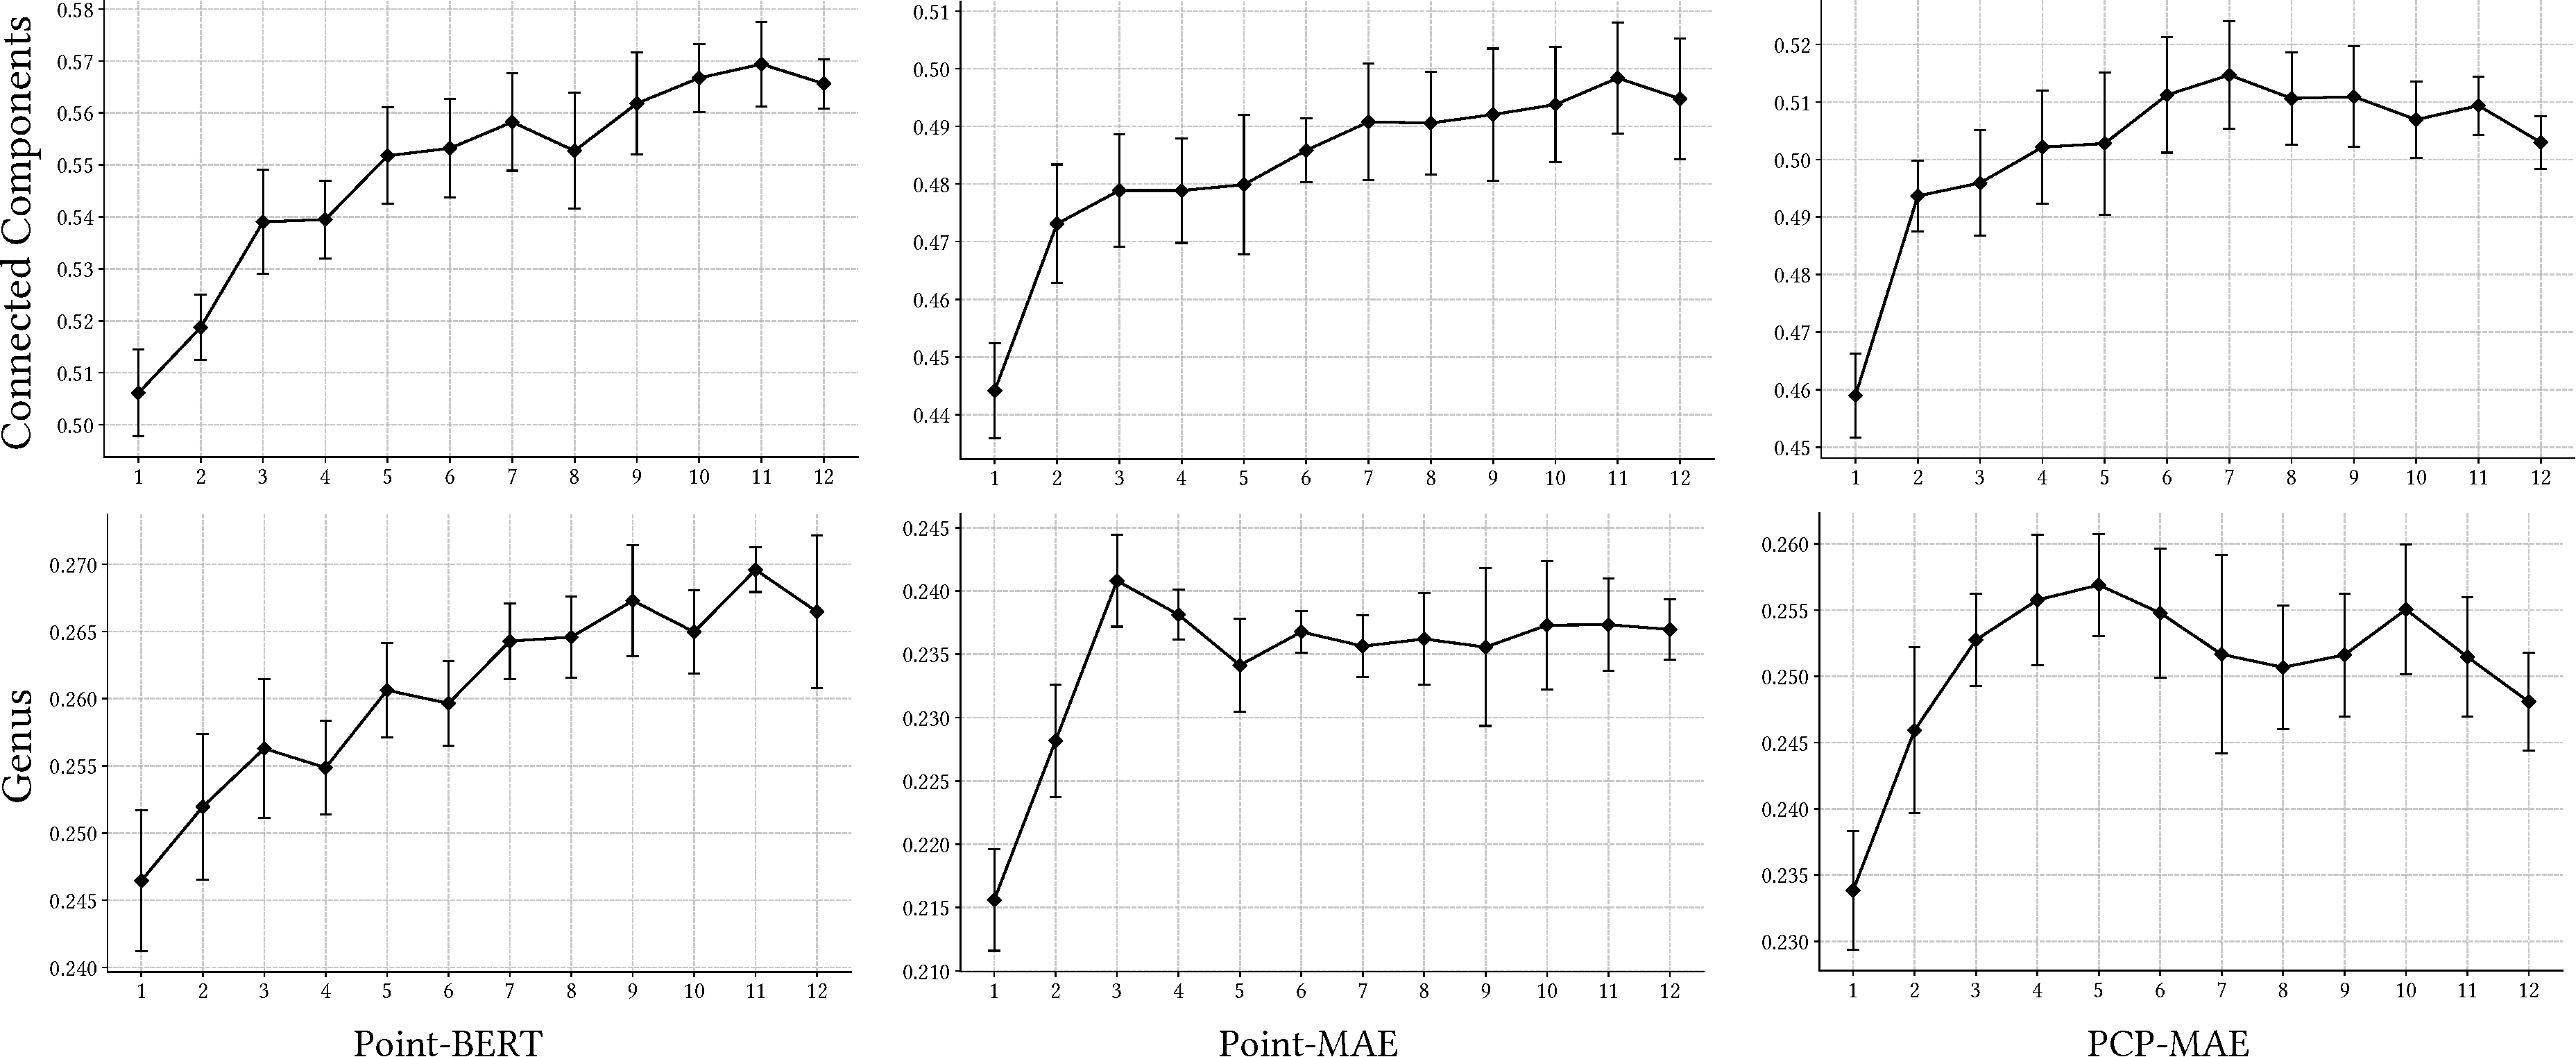
\includegraphics[width=\linewidth]{figs/probing.pdf}
  \caption{\textbf{Linear probing accuracy across transformer layers for Point-BERT (left column) and Point-MAE (right column).} We report probing accuracy for connected components (top row) and genus (bottom row). For each setting, accuracy values are averaged over the validation sets from a 5-fold cross-validation procedure, with error bars representing the corresponding standard deviations. For Point-BERT, probing is applied to the CLS token, which aggregates global information throughout the network. For Point-MAE, which does not include a CLS token during pretraining, we instead use the max-pooled patch embeddings from each layer.}
  \label{fig:probing-results}
\end{figure}

We start by probing transformer models to assess whether their internal representations encode information about shape topology. Specifically, we test if simple linear classifiers can recover the genus and number of connected components of shapes from the DONUT dataset using the representations of each intermediate layer. This approach provides a first estimate of how topological signals are distributed across the model depth.

\paragraph{Motivation.}
Linear probing is a standard approach in representation learning to evaluate how much a given factor of variation is linearly accessible from the learned embeddings. It assumes that if a linear classifier performs well, the corresponding information is already represented in a linearly separable manner. Importantly, several works have shown that the most informative representations for downstream tasks are not always located in the final layers of a model. Intermediate layers can encode more general or transferable structures before they are transformed into task-specific representations. This has been established in both vision and language transformers~\cite{intermediate_layers, structural_probe, vit_probing}. We therefore analyze not only the final layer, but the entire depth of each model, to capture where topology-related features emerge.

\paragraph{Experimental setup.}
For each evaluated model, we freeze the pretrained backbone and extract offline activations from all transformer layers on the DONUT dataset. At every layer $l$, we train two separate linear classifiers on top of the frozen representations to predict (i) the genus and (ii) the number of connected components. We perform 5-fold cross-validation and report averaged accuracy on the validation set.

\paragraph{Results.}
Overall, Figure~\ref{fig:probing-results} probing accuracy tends to increase with network depth for both models, indicating that higher transformer layers capture richer structural information. The improvement is modest for genus prediction, with an average increase of about 3\% between the first and last layers. In contrast, connected component prediction improves by roughly 8\%, suggesting that the notion of component separation becomes more explicit as features become increasingly global. This aligns with the expectation that transformers progressively aggregate local patch information into holistic shape-level representations.

Interestingly, in Point-MAE, accuracy for genus prediction plateaus after layer 5. This saturation may reflect the limited capacity of shallow hierarchies to encode topological invariants that depend on multi-scale relationships between local patches. Testing deeper or hierarchical variants of Point-MAE could help determine whether such information emerges later in the network.

Despite these relative improvements, absolute scores remain low: around 20\% for genus and 50\% for connected components, highlighting that both models only weakly encode topology. This supports the view that current pretraining objectives, which focus on geometric reconstruction or semantic alignment, do not drive models to capture global connectivity. While deeper layers improve aggregation and invariance, they remain sensitive to geometric details rather than structural invariants. These results reinforce that topology-aware objectives or explicit topological supervision may be required to make 3D encoders truly aware of shape structure beyond geometry.

\subsection{Subspace Alignment with Persistent Homology}
\label{ssec:ph}

\begin{figure}[h]
  \centering
  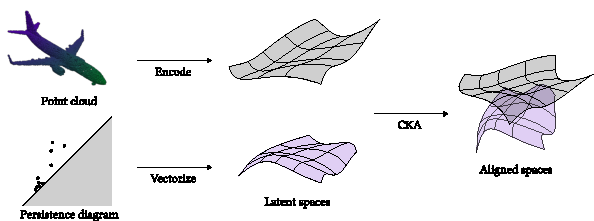
\includegraphics[width=\linewidth]{figs/alignment.pdf}
  \caption{\textbf{Alignment procedure overview.} We extract features from a 3D point cloud with the model we seek to evaluate. We also vectorize its corresponding persistence diagram (Section~\ref{sssec:vectorization_persistence_diagrams}). We then compute the CKA similarity (Section~\ref{sssec:subspace_alignment_protocol}) between the two sets of features to quantify how well the learned representation aligns with topological signatures.}
  \label{fig:alignment}
\end{figure}

We study the relationship between representations learned by 3D shape encoders and those derived from persistent homology. Following the perspective of the Platonic Representation Hypothesis~\cite{plato,platonic}, we view learned embeddings as potentially containing subspaces that capture intrinsic structural information. Information captured by persistent homology can also be treated as a complementary modality. Assuming there's a way to encode topological features into a vector space, we can then ask whether the learned and topological subspaces align. It's worth noticing that the analogy with \cite{platonic} is not perfect: while it's assumed that representations tend to converge at scale, topological features, even learned ones, aren't the result of large scale training.

We first review background on persistent homology and its vectorization. We then formally define the metrics used to quantify alignment. Finally, we describe our alignment protocol and present results across encoders and datasets.


\subsubsection{Persistence Diagrams}
\label{sssec:persistence_diagrams}


\paragraph{Filtrations.}
Let $(X, \leq)$ be a topological space equipped with a real index. A (real) filtration is a family of subspaces $(X_a)_{a\in\mathbb{R}}$ with $X_a \subseteq X_b$ whenever $a \leq b$ and $\bigcup_a X_a = X$. Typical examples are sublevel sets of a function $f:X\to\mathbb{R}$, namely $X_a = f^{-1}((-\infty,a])$.

\paragraph{Homology and persistent maps.}
Fix a field $\Bbbk$ and compute singular or simplicial homology with coefficients in $\Bbbk$. For $k\ge 0$ and $a\le b$, the inclusion $X_a \hookrightarrow X_b$ induces a linear map
\begin{equation}
i_{a}^{b}: H_k(X_a;\Bbbk) \longrightarrow H_k(X_b;\Bbbk).
\end{equation}
A $k$-dimensional class $\alpha\in H_k(X_b)$ is \emph{born} at the smallest $a$ for which it has a representative in $H_k(X_a)$, and it \emph{dies} at the smallest $d>b$ where it maps to zero in $H_k(X_d)$ under $i_{b}^{d}$. Classes that never die are called \emph{essential}.

\paragraph{Persistence modules, barcodes and diagrams.}
The collection $\{H_k(X_a), i_{a}^{b}\}_{a\le b}$ is a persistence module. Under standard finiteness conditions (e.g. $f$ tame, or finite type filtrations), it decomposes into interval modules. This gives a multiset of intervals (the barcode) or equivalently a multiset of points $(b_i,d_i)$ in the open half plane $\{(x,y)\in\mathbb{R}^2: x<y\}$ together with the diagonal $\{(t,t)\}$ available for matching with infinite multiplicity. This multiset is the $k$-th persistence diagram $\mathrm{Dgm}_k(X)$.

\paragraph{Why a persistence diagram is not a Euclidean vector object.}
A persistence diagram is a collection of points in the plane, where each point $(b,d)$ records the birth and death of a topological feature during a filtration. Points on the diagonal $(b=d)$ correspond to features that disappear immediately, and we assume there are infinitely many of them so that every feature in one diagram can be matched to a trivial one in another when comparing diagrams. Unlike vectors in Euclidean space, persistence diagrams cannot be naturally added or scaled, since such operations would destroy their topological meaning. Even computing an average of several diagrams can give multiple different results. In some cases, a diagram may even have infinitely many points away from the diagonal if the underlying space behaves badly. Therefore, persistence diagrams are treated as elements of a metric space, with distances defined by measures such as the bottleneck or Wasserstein metric, rather than as vectors in a linear space.

\paragraph{Distances between diagrams.}
Let $D$ and $E$ be diagrams. We allow matchings to the diagonal. The \emph{bottleneck distance} is
\begin{equation}
d_B(D,E) \;=\; \inf_{\gamma:D\to E} \; \sup_{x\in D} \, \lVert x - \gamma(x) \rVert_{\infty}.
\end{equation}
For $1\le p<\infty$, the $p$-\emph{Wasserstein distance} is
\begin{equation}
d_{W,p}(D,E) \;=\; \left( \inf_{\gamma:D\to E} \; \sum_{x\in D} \lVert x - \gamma(x) \rVert_{\infty}^{\,p} \right)^{1/p}.
\end{equation}
These are the standard and stable distances on persistence diagrams. The plain Hausdorff distance between the underlying point sets does not account for multiplicities and diagonal matchings and is not used in modern stability theory.

\paragraph{Stability theorems.}
For sublevel set filtrations of functions $f,g:X\to\mathbb{R}$ on a common triangulable space, the diagrams are stable under perturbations of $f$:
\begin{equation}
d_B\big(\mathrm{Dgm}_k(f), \mathrm{Dgm}_k(g)\big) \;\le\; \lVert f-g \rVert_{\infty}.
\end{equation}
Related bounds hold for $d_{W,p}$. In the algebraic language of persistence modules, the Isometry Theorem states that for $q$-tame modules $M,N$,
\begin{equation}
d_B\big(\mathrm{Dgm}(M), \mathrm{Dgm}(N)\big) \;=\; d_I(M,N),
\end{equation}
where $d_I$ is the interleaving distance.


\begin{figure}[t]
  \centering
  % Top full-width subfigure
  \begin{subfigure}{\linewidth}
    \centering
    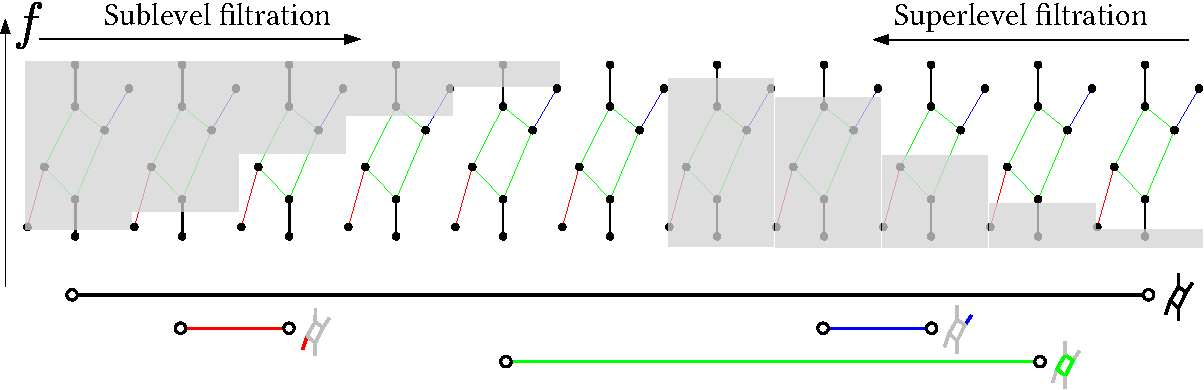
\includegraphics[width=\linewidth]{figs/ph/expers_v2.pdf}
    \caption{Sub- (resp. super-) level set filtration.}
    \label{fig:filtrations_top}
  \end{subfigure}

  \vspace{0.5em} % space between top and bottom row

  % Bottom two subfigures
  \begin{subfigure}{0.48\linewidth}
    \centering
    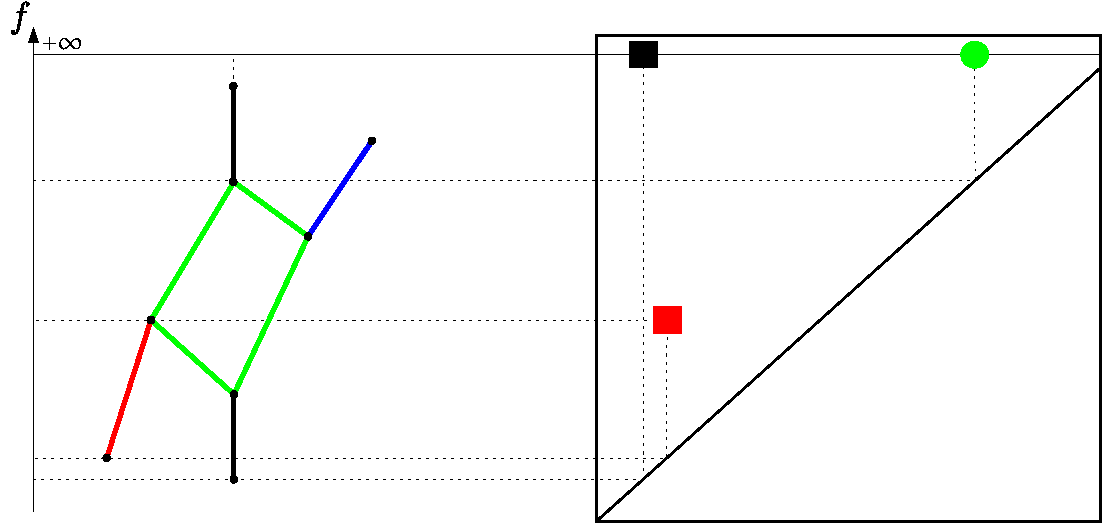
\includegraphics[width=\linewidth]{figs/ph/expers2_ord_v2.pdf}
    \caption{Ordinary persistence diagram.}
    \label{fig:filtrations_left}
  \end{subfigure}\hfill
  \begin{subfigure}{0.48\linewidth}
    \centering
    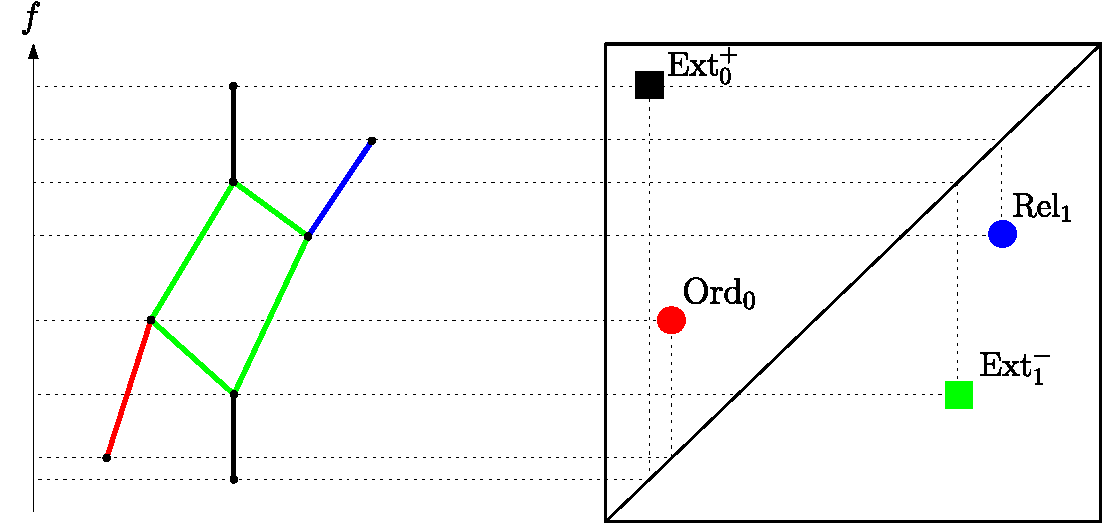
\includegraphics[width=\linewidth]{figs/ph/expers2_v2.pdf}
    \caption{Extended persistence diagram.}
    \label{fig:filtrations_right}
  \end{subfigure}

  \caption{\textbf{Ordinary vs extended persistence.} (Figures adapted from \cite{perslay}). In \ref{fig:filtrations_top}, each node of the graph is assigned its height. Persistence intervals are shown under the sequence. In \ref{fig:filtrations_left}, ordinary persistence captures connected components and loops, but essential classes lead to infinite intervals (black and green markers) and the upward branch (blue) isn't captured. In \ref{fig:filtrations_right}, extended persistence pairs all classes at finite values by combining sublevel and superlevel filtrations with relative homology. Finally, $\text{Ext}_0^+$, $\text{Ext}_1^-$, $\text{Ord}_0$ and $\text{Ord}_1$ denote the different types of pairs in extended persistence.}
  \label{fig:filtrations}
\end{figure}


\paragraph{Extended persistence.}
Essential classes can lead to pairs with infinite lifetime. Extended persistence remedies this by combining sublevel and superlevel filtrations and using relative homology. For a function $f:X\to\mathbb{R}$ on a compact space, consider the sublevel filtration $(X_a)$ and the superlevel filtration $(X^a = f^{-1}([a,\infty)))$. One constructs a zigzag that passes from absolute to relative homology so that every class is paired at a finite parameter value. The resulting \emph{extended persistence diagram} has only finite pairs and encodes essential features as finite points. Figure~\ref{fig:filtrations} illustrates the filtration process as well as the difference between ordinary and extended persistence on a simple graph.


\subsubsection{Vectorization of Persistence Diagrams}
\label{sssec:vectorization_persistence_diagrams}

\begin{figure}[t]
    \centering
    \begin{subfigure}[b]{0.23\textwidth}
        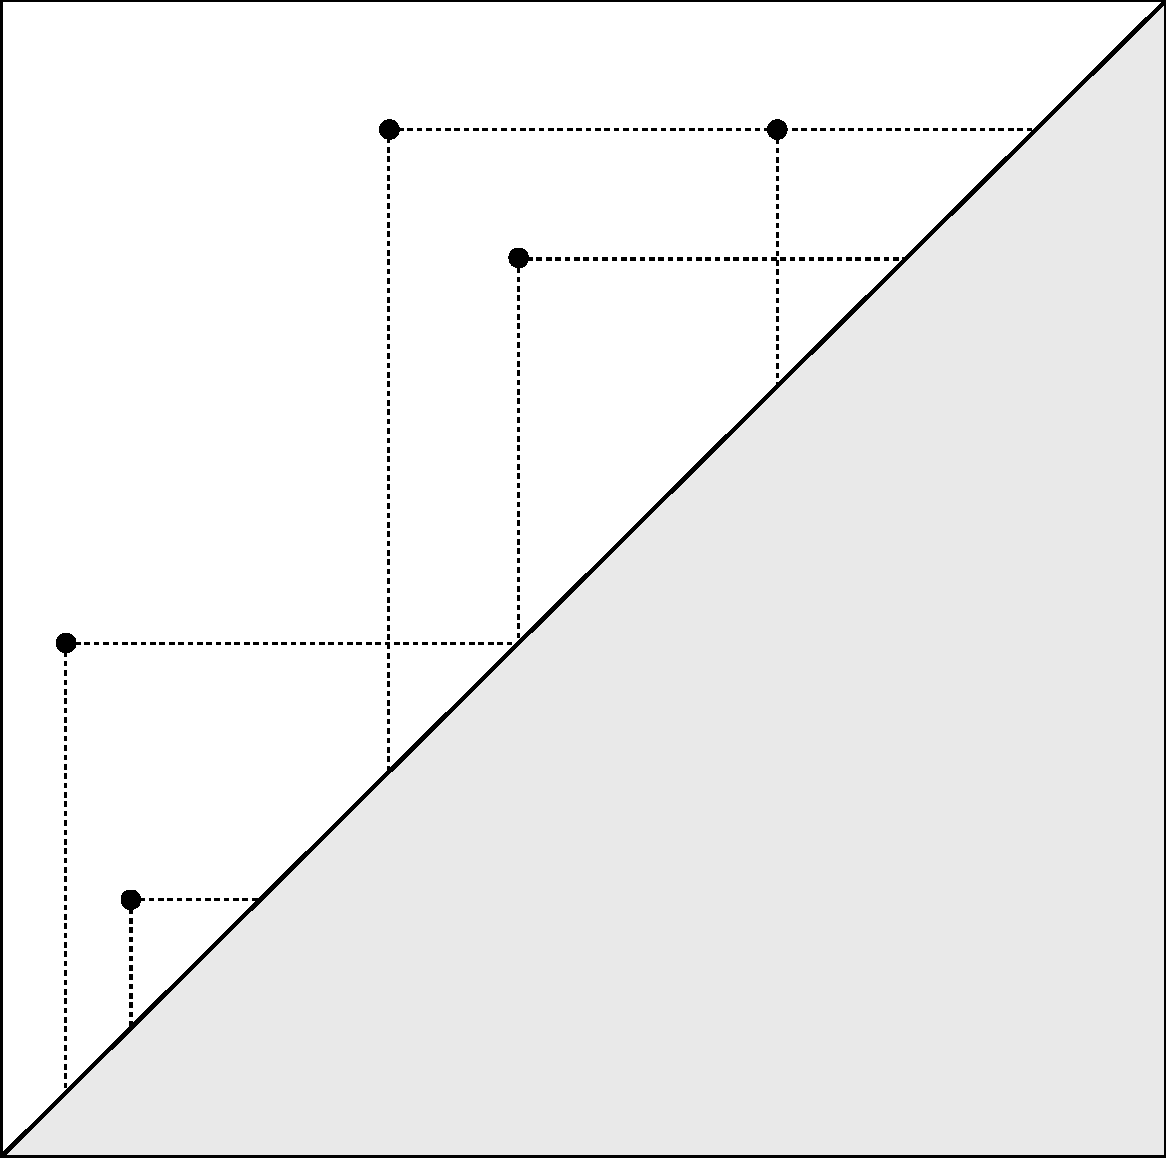
\includegraphics[width=\textwidth]{figs/ph/examples/pd_example.pdf}
        \caption{Persistence Diagram}
    \end{subfigure}\hfill
    \begin{subfigure}[b]{0.23\textwidth}
        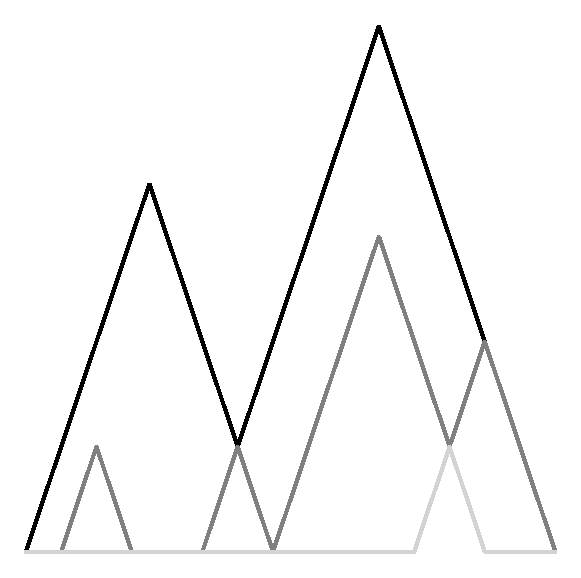
\includegraphics[width=\textwidth]{figs/ph/examples/landscape_example.pdf}
        \caption{Persistence Landscape}
    \end{subfigure}\hfill
    \begin{subfigure}[b]{0.23\textwidth}
        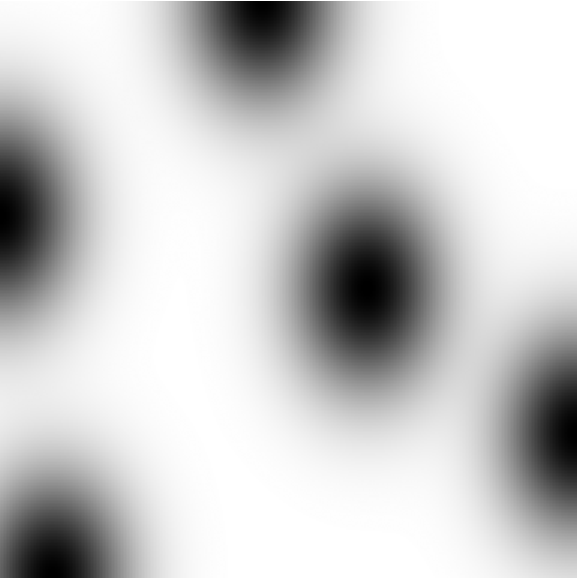
\includegraphics[width=\textwidth]{figs/ph/examples/persistence_image_example.pdf}
        \caption{Persistence Image}
    \end{subfigure}\hfill
    \begin{subfigure}[b]{0.23\textwidth}
        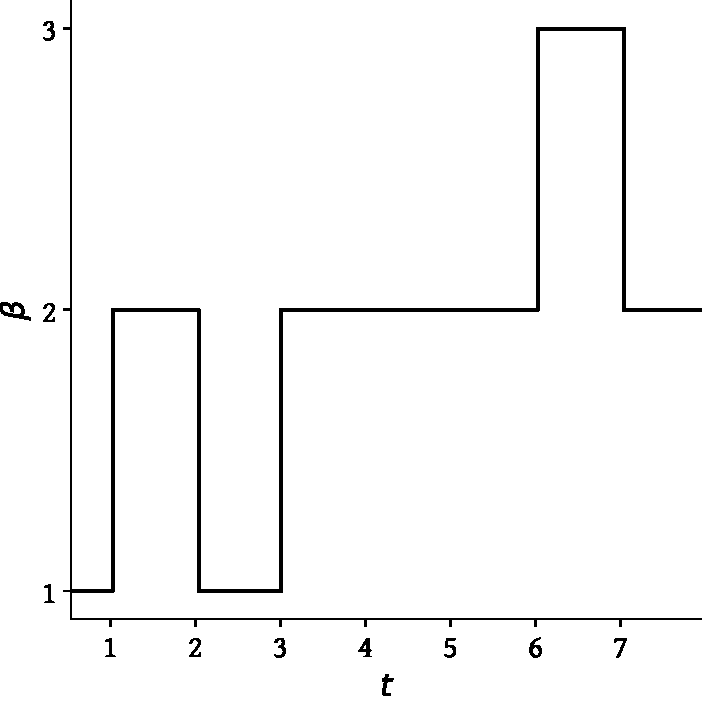
\includegraphics[width=\textwidth]{figs/ph/examples/betti_curve_example.pdf}
        \caption{Betti Curve}
    \end{subfigure}
    \caption{\textbf{Common prescribed vectorizations of a persistence diagram.} From left to right: (a) A sample persistence diagram with points representing topological features; (b) Persistence landscape capturing the prominence of features across scales; (c) Persistence image providing a smoothed, grid-based representation; \textit{Note:} Instead of considering persistence pairs as a \textit{(birth,death)} tuple, persistence image is fitted on $(birth, death-birth)$ pairs. (d) Betti curve showing the count of features over filtration values.}
    \label{fig:ph-vectorizations}
\end{figure}

Vectorizing persistence diagrams is crucial for incorporating topological signals in standard learning pipelines. A persistence diagram is a multiset of points in the plane. It does not live in a vector space and is usually compared with bottleneck or Wasserstein distances rather than inner products. Most learning algorithms expect fixed size vectors or a Hilbert space structure, so raw diagrams are not a natural input. Diagrams also have variable size and are permutation invariant, which complicates batching and optimization. These issues motivate stable feature maps and kernels that embed diagrams into Euclidean 

\textbf{Prescribed Vectorization.} Handcrafted summaries (Figure~\ref{fig:ph-vectorizations}) have long been the dominant strategy for vectorizing persistence diagrams in machine learning. The most common approaches include persistence landscapes \cite{persistence_landscapes}, Betti curves \cite{betti_curves}, and persistence images \cite{persistence_images} (Figure~\ref{fig:ph-vectorizations}). Landscapes embed diagrams in a Hilbert space and enable classical statistics, but they still require design choices such as the number of landscape levels and sampling resolution. Betti curves collapse a diagram to simple counting functions over the filtration. Persistence images rasterize diagrams with a kernel on a fixed grid. These methods are stable in theory but depend on key hyperparameters such as grid resolution and kernel width. These choices must be tuned per task and can limit expressiveness and generalization. Finally, ATOL \cite{atol} proposes an unsupervised alternative. It vectorizes measures, including sets of persistence points, by first clustering with K-means and then summarizing cluster statistics in a fixed length descriptor. The pipeline is simple and fast but remains sensitive to the chosen number of clusters and to the distribution shift between training and test diagrams.

\textbf{Learned Vectorization.} Recent work has moved from handcrafted features to learning based approaches \cite{adaptive_topological_feature},\cite{topological_signature} that act on persistence diagrams more directly, often through extended persistence \cite{extended_persistence} (see Section ...). PersLay \cite{perslay} introduces a neural layer that learns stable weights and pooling functions over points in a diagram. It was developed for graph tasks and relies on extended persistence to encode informative signatures before the learned aggregation. PLLay \cite{pllay} follows a hybrid route. It first computes persistence landscapes and then applies a differentiable neural layer that learns how to weight and combine landscape coordinates. This reduces manual feature design while keeping the stability benefits of landscapes. Transformer based designs have also appeared. Persformer \cite{persformer} treats each persistence point as a token and applies standard self attention. This is flexible but scales poorly as the number of points grows. To address scalability, the Multiset Transformer \cite{multiset_transformer} clusters points and modifies attention to account for multiplicities, so that a cluster can be handled as a single item with weight greater than one. This change reduces memory and time while preserving permutation invariance at the multiset level. xPerT \cite{xpert} goes further by leveraging sparsity with a \textit{pixelized diagram} representation. It is close in spirit to persistence images but does not require a smoothing kernel. The pixeliaation allows efficient tokenization and improves scalability compared with Persformer. xPerT also works with extended persistence; details are deferred to the dedicated section.

Across these learning based methods, a common trait is that the diagram is manipulated explicitly rather than replaced by coarse handcrafted summaries. Most results to date are on graph benchmarks rather than 3D shape understanding. This gap limits conclusions for point cloud encoders trained in a self supervised way, where task independent evaluation is required.

Finally, recent topology aware 3D generation pipelines \cite{topology_aware_latent_diffusion} directly encode persistence pairs. More precisely they feed the top k most persistent pairs as $\{g_i=(b_i, d_i-b_i)\}_{i \in \llbracket 1,k\rrbracket}$ where $b_i$ is the birth time and $d_i$ is the death time of the i-th pair. These papers report increased diversity or topology control but are typically demonstrated on a few ShapeNet categories or related datasets. A representative example conditions a latent diffusion model on topological features computed from persistence diagrams and validates on ShapeNet and ABC.

\subsubsection{Subspace Alignment Protocol}
\label{sssec:subspace_alignment_protocol}

\paragraph{Background}
To assess whether a learned 3D encoder’s internal representations align with topological signatures derived from persistent homology, we adopt Centered Kernel Alignment (CKA) as our similarity metric. CKA has become a standard tool in recent work for comparing internal neural representations, because it overcomes certain limitations of canonical correlation analysis (CCA) in high-dimensional settings and provides a normalized similarity score between two representational spaces \cite{cka}.

Let $X\in \mathbb{R}^{n \times d_X}$ and $Y\in \mathbb{R}^{n \times d_Y}$ be two sets of centered features across $n$ examples (rows). We form Gram (kernel) matrices $K = X X^\top$ and $L = Y Y^\top$. Let $H = I_n - \frac1n \mathbf{1}\mathbf{1}^\top$ be the centering matrix. The (biased) Hilbert–Schmidt independence measure is: 

\begin{equation}
\mathrm{HSIC}(K,L) = \frac{1}{(n-1)^2} \mathrm{trace}(KHLH).
\end{equation}

The CKA similarity is then defined as:

\begin{equation}
\mathrm{CKA}(X,Y) = \frac{\mathrm{HSIC}(K,L)}{\sqrt{\mathrm{HSIC}(K,K) \mathrm{HSIC}(L,L)}}.
\end{equation}

This normalization ensures that $\mathrm{CKA}(X,Y)\in [0,1]$ and is invariant to isotropic scaling of features. An unbiased estimator of HSIC can also be used to mitigate bias induced by finite samples or mini-batching.

We choose CKA for several reasons. First, its normalization makes the similarity more interpretable across different layer sizes or vectorization dimensions. Second, in empirical studies, CKA has proven effective at identifying correspondences between layers of differently initialized or architected networks (while pure CCA-type metrics sometimes fail). Third, because it works by comparing inner-product (kernel) structures, it is well suited to capture alignment between representational geometries rather than mere coordinate-wise correlation. Finally, in our context, since the topological encoding (via vectorized persistence diagrams) and the learned features live in distinct vector spaces, using a kernel-based alignment provides a flexible and robust way to detect shared structure, even if the bases or dimensions differ.

Thus in our protocol, we treat a vectorization of the persistence diagram as one representational matrix $Y$, and the activations extracted from a given layer of the 3D encoder as $X$. Then we compute $\mathrm{CKA}(X,Y)$ to quantify how well that encoder subspace aligns with the topological modality.

\paragraph{Experimental setting.}



\paragraph{Results}
To be completed.

\subsection{Changing the Pretraining Data Distribution}
\label{ssec:changing_pretraining_data_distribution}

\begin{figure}[h]
  \centering
  
  \includegraphics[width=\linewidth]{figs/reconstruction.pdf}
  \caption{\textbf{Point-cloud reconstruction for different encoders.} Each pretrained model is fed with a point cloud with 2048 points. We reconstruct it with the decoder used during pretraining with a masking ratio of zero. To ensure topological structures of the input are captured, we patchify the input point cloud into overlapping local regions before encoding, and decode to a reconstructed point cloud of 4096 points. Reconstructed point-clouds don't exhibit the 3 characteristic holes of the input shape.}
  \label{fig:reconstructions}
\end{figure}


Previous experiments showed that current 3D encoders have a limited understanding of topological structures. This section investigates a simple hypothesis. In data-driven approaches, models learn to extract information that is relevant to the pretraining objective. All the considered encoders are pretrained on reconstruction tasks using the Chamfer loss. These tasks rely only on geometric proximity between predicted and target point clouds, without explicitly rewarding structural consistency. Moreover, the pretraining data itself lacks topological diversity. Datasets such as ShapeNet mostly contain single, compact objects with few or no holes. As a result, encoders can achieve low reconstruction errors without learning to capture non-trivial topological properties. This experiment is further motivated by Figure~\ref{fig:reconstructions}, which shows that pretrained encoders struggle to reconstruct even simple topological structures.

\begin{table}
% \renewcommand\arraystretch{1.2}
\begin{center}
\begin{tabular}{l|ccc}
    
\toprule
Method & OBJ-BG & OBJ-ONLY & PB-T50-RS \\
% \cmidrule(lr){2-5} \cmidrule(lr){6-9}
\midrule

Point-BERT~\cite{pbert} & 87.43 & 88.12 & 83.07\\
Point-BERT (ABC) & 88.30 & 88.47 & 83.55 \\
\textit{difference} & \cellcolor{green!25}$+0.87$ & \cellcolor{green!25}$+0.35$ & \cellcolor{green!25}$+0.48$ \\
\midrule
Point-MAE~\cite{pmae} & 90.02 & 88.29 & 85.18 \\
Point-MAE (ABC) & 88.64 & 88.47 & --\\
\textit{difference} & \cellcolor{orange!25}$-1.38$ & \cellcolor{green!25}$+0.18$ & --\\
\midrule
PM2AE~\cite{pm2ae} & 91.22 & 88.81 & 86.43 \\
PM2AE (ABC) & 90.02 & 89.67 & -- \\
\textit{difference} & \cellcolor{orange!25}$-1.2$ & \cellcolor{green!25}$+0.86$ & -- \\
\midrule
PCP-MAE~\cite{pcpmae} & -- & -- & -- \\
PCP-MAE (ABC) & -- & -- & -- \\
\textit{difference} & -- & -- & -- \\

\bottomrule
\end{tabular}
\caption{{\bf Classification results on ScanObjectNN.} For each backbone model, we compare performance when pretrained on ShapeNet (first row) versus ABC (second row). The third row shows the difference, with green indicating improvement and orange indicating decline when using ABC.}
\setlength\tabcolsep{2pt}
\label{tb:scanobject}
\end{center}

\end{table}
We hypothesize that changing the pretraining data distribution can improve the model's structural understanding. By exposing encoders to shapes with richer and more diverse topology, they may learn internal representations that better capture global structure. To test this idea, we pretrain all the previously evaluated encoders on the ABC dataset. This dataset contains CAD models with a wide range of geometric and topological configurations. For a fair comparison with models pretrained on ShapeNet, which contains 51K samples, we randomly select 55K shapes from ABC. We strictly follow the same pretraining procedure, including the reconstruction objective and optimization settings.

To evaluate this hypothesis, we assess two key aspects: (1) whether the models retain their performance on standard downstream tasks, and (2) whether they show improved structural understanding. We follow the evaluation protocols introduced in the original papers of each encoder.

\paragraph{Object Classification.}
We first verify that pretraining on ABC does not degrade general performance on standard semantic tasks. Object classification is performed on the ScanObjectNN dataset, a real-world benchmark built from scanned indoor objects. It contains 15,000 samples across 15 categories, organized into three variants of increasing difficulty: obj only, which includes cleanly segmented objects; obj bg, where background points are kept; and PB T50 RS, which introduces heavy noise and random perturbations. This dataset is considered challenging because it captures real-world imperfections such as occlusions and partial views, unlike synthetic datasets like ShapeNet.

As shown in Table~\ref{tb:scanobject}, models pretrained on ABC perform similarly or slightly better than those pretrained on ShapeNet. This suggests that changing the pretraining distribution to CAD models whose semantic content differs from the finetuning dataset does not harm performance on semantic classification. In fact, exposure to a more topologically varied pretraining set may even promote better generalization.


\begin{table}
% \renewcommand\arraystretch{1.2}
\begin{center}
\begin{tabular}{l|cccc|cccc}
    
\toprule
& \multicolumn{4}{c|}{\textbf{ModelNet}} & \multicolumn{4}{c}{\textbf{DONUT (genus)}} \\
% \cmidrule(lr){2-5} \cmidrule(lr){6-9}
& \multicolumn{2}{c}{5-way} & \multicolumn{2}{c|}{10-way} & \multicolumn{2}{c}{5-way} & \multicolumn{2}{c}{10-way} \\
\cmidrule(lr){2-3} \cmidrule(lr){4-5} \cmidrule(lr){6-7} \cmidrule(lr){8-9}
Methods & 10-shot & 20-shot & 10-shot & 20-shot & 10-shot & 20-shot & 10-shot & 20-shot \\
\midrule

Point-BERT~\cite{pbert} & $94.6_{\pm 3.1}$ & $96.3_{\pm 2.7}$ & $91.0_{\pm 5.4}$ & $92.7_{\pm 5.1}$ & -- & -- & -- & --\\
Point-BERT (ABC) & $95.9_{\pm 2.1}$ & $98.1_{\pm 1.8}$ & $91.7_{\pm 4.5}$ & $94.2_{\pm 3.4}$ & -- & -- & -- & --\\
\midrule
Point-MAE~\cite{pmae} & $96.3_{\pm 2.5}$ & $97.8_{\pm 1.8}$ & $92.6_{\pm 4.1}$ & $95.0_{\pm 3.0}$ & $32.9_{\pm 3.5}$ & $38.1_{\pm 3.9}$ & $20.4_{\pm 2.1}$ & $23.8_{\pm 1.7}$ \\
Point-MAE (ABC) & $96.2_{\pm 2.7}$ & $97.6_{\pm 1.9}$ & $92.3_{\pm 4.4}$ & $95.2_{\pm 2.9}$ & $35.1_{\pm 6.0}$ & $40.1_{\pm 4.9}$ & $21.4_{\pm 2.7}$ & $22.8_{\pm 2.4}$\\
\textit{difference} & \cellcolor{orange!25}$-0.1$ & \cellcolor{orange!25}$-0.2$ & \cellcolor{green!25}$+0.3$ & \cellcolor{green!25}$+0.2$ & \cellcolor{green!25}$+2.2$ & \cellcolor{green!25}$+2.0$ & \cellcolor{green!25}$+1.0$ & \cellcolor{orange!25}$-1.0$ \\
\midrule
PM2AE~\cite{pm2ae} & $96.8_{\pm 1.8}$ & $98.3_{\pm 1.4}$ & $92.3_{\pm 4.5}$ & $95.0_{\pm 3.0}$ & $34.7_{\pm 4.2}$ & $41.8_{\pm 6.3}$ & $21.2_{\pm 2.2}$ & $25.0_{\pm 1.3}$\\
PM2AE (ABC) & $95.9_{\pm 2.4}$ &$97.7_{\pm 1.8}$ & $91.1_{\pm 4.6}$ & $94.4_{\pm 3.4}$ & $37.0_{\pm 4.7}$ & $43.4_{\pm 5.3}$ & $22.8_{\pm 1.7}$ & $26.3_{\pm 2.3}$\\
\textit{difference} & \cellcolor{orange!25}$-0.9$ & \cellcolor{orange!25}$-0.6$ & \cellcolor{orange!25}$-1.2$ & \cellcolor{orange!25}$-0.6$ & \cellcolor{green!25}$+2.3$ & \cellcolor{green!25}$+1.8$ & \cellcolor{green!25}$+1.6$ & \cellcolor{green!25}$+1.3$ \\
\midrule
PCP-MAE~\cite{pcpmae} & $97.4_{\pm 2.3}$ & $99.1_{\pm 0.8}$ & $93.5_{\pm 3.7}$ & $95.9_{\pm 2.7}$ & $36.6_{\pm 5.4}$ & $41.8_{\pm 4.0}$ & $21.5_{\pm 2.0}$ & $24.6_{\pm 1.7}$\\
PCP-MAE (ABC) & $96.1_{\pm 3.1}$ & $98.3_{\pm 4.3}$ & $91.7_{\pm 4.3}$ & $94.9_{\pm 2.9}$ & $38.7_{\pm 4.2}$ & $44.5_{\pm 5.4}$ & $22.4_{\pm 1.9}$ & $26.0_{\pm 1.4}$\\
\textit{difference} & \cellcolor{orange!25}$-1.3$ & \cellcolor{orange!25}$-0.8$ & \cellcolor{orange!25}$-1.8$ & \cellcolor{orange!25}$-1.0$ & \cellcolor{green!25}$+2.1$ & \cellcolor{green!25}$+2.7$ & \cellcolor{green!25}$+0.9$ & \cellcolor{green!25}$+1.4$ \\

\bottomrule
\end{tabular}
\caption{{\bf Few-shot object classification on ModelNet40.} We conduct 10 independent experiments for each setting and report mean accuracy (\%) with standard deviation.}
\setlength\tabcolsep{2pt}
\label{tb:few}
\end{center}

\end{table}
\paragraph{Few-Shot Classification.}
We further evaluate the learned representations under few-shot settings. Following the standard protocol, we perform few-shot classification on ModelNet40, which contains 12,311 clean CAD models from 40 categories, and on DONUT, which includes point clouds with richer topology, such as multiple connected components and non-trivial holes. Few-shot experiments are conducted with 5 or 10 ways (number of selected categories), 10 or 20 shots (number of samples per class), and tested on 20 samples per class.

Results in Table~\ref{tb:few} show that performance on ModelNet40 remains close across both pretraining datasets, while models pretrained on ABC consistently achieve better results on DONUT (except for the 10-way 20-shot setting on Point-MAE). The overall low accuracy on DONUT, however, confirms that this task remains non-trivial and highlights the current models’ limited structural understanding.
